\documentclass[a4paper,10pt]{article}
\usepackage[paper=a4paper, hmargin=1.5cm, bottom=1.5cm, top=3.5cm]{geometry}
\usepackage[latin1]{inputenc}
\usepackage[T1]{fontenc}
\usepackage[spanish]{babel}
\usepackage{amssymb}
\usepackage{amsmath}
\usepackage{mathtools}
\usepackage{fancyhdr}
\usepackage{lastpage}
\usepackage{caratula}
\usepackage{verbatim}
\usepackage{xspace}
\usepackage{xargs}
\usepackage{float}
\usepackage{graphicx}
\usepackage{ifthen}
\usepackage[spanish,noline,longend]{algorithm2e}
\usepackage{listings}
\usepackage{braket}
%\usepackage{aed2-tad,aed2-symb,aed2-itef}

\lstset{language=C++, tabsize=4, breaklines=true, breakatwhitespace=true, numbers=left, numbersep=10pt}

\newcommand{\moduloNombre}[1]{\textbf{#1}}

\let\NombreFuncion=\textsc
\let\TipoVariable=\texttt
\let\ModificadorArgumento=\textbf
\newcommand{\res}{$res$\xspace}
\newcommand{\tab}{\hspace*{7mm}}

\newcommandx{\TipoFuncion}[3]{%
  \NombreFuncion{#1}(#2) \ifx#3\empty\else $\to$ \res\,: \TipoVariable{#3}\fi%
}
\newcommandx{\Pre}[1][1=true]{\textbf{Pre} $\equiv$ \{#1\}\\}
\newcommand{\Post}[1]{\textbf{Post} $\equiv$ \{#1\}}
\newcommand{\In}[2]{\ModificadorArgumento{in} \ensuremath{#1}\,: \TipoVariable{#2}\xspace}
\newcommand{\Out}[2]{\ModificadorArgumento{out} \ensuremath{#1}\,: \TipoVariable{#2}\xspace}
\newcommand{\Inout}[2]{\ModificadorArgumento{in/out} \ensuremath{#1}\,: \TipoVariable{#2}\xspace}
\newcommand{\Aplicar}[2]{\NombreFuncion{#1}(#2)}

\newlength{\IntFuncionLengthA}
\newlength{\IntFuncionLengthB}
\newlength{\IntFuncionLengthC}
%InterfazFuncion(nombre, argumentos, valor retorno, precondicion, postcondicion, complejidad, descripcion, aliasing)
\newcommandx{\InterfazFuncion}[9][4=true,6,7,8,9]{%
  \hangindent=\parindent
  \TipoFuncion{#1}{#2}{#3}\\%
%  \textbf{Pre} $\equiv$ \{#4\}\\%
%  \textbf{Post} $\equiv$ \{#5\}%
  \Pre[#4]
  \Post{#5}
  \ifx#6\empty\else\\\textbf{Complejidad:} #6\fi%
  \ifx#7\empty\else\\\textbf{Descripci�n:} #7\fi%
  \ifx#8\empty\else\\\textbf{Aliasing:} #8\fi%
  \ifx#9\empty\else\\\textbf{Requiere:} #9\fi%
}



\newenvironment{Interfaz}{%
  \parskip=2ex%
  \noindent\textbf{\Large Interfaz}%
  \par%
}{}

\newcommand{\Forcond}[2]{
  #1 \textbf{to} #2
}

\newenvironment{Representacion}{%
  \vspace*{2ex}%
  \noindent\textbf{\Large Representaci�n}%
  \vspace*{2ex}%
}{}

\newenvironment{Algoritmos}{%
  \vspace*{2ex}%
  \noindent\textbf{\Large Algoritmos}%
  \vspace*{2ex}%
}{}

%
%\newcommandx{\Signatura}[3][3]{%
%  \NombreFuncion{#1}(#2)
%  \ifx#3\empty\else $\to$ \res\,: \TipoVariable{#3}\fi
%  \\
%}


\newenvironmentx{algoritmo}[6][3,4,5,6]{
  \begin{algorithm}[H]
  \DontPrintSemicolon
  \newcommandx{\Signatura}[3][3]{
    \NombreFuncion{##1}(##2)
    \ifx##3\empty\else $\to$ \res\,: \TipoVariable{##3}\fi
    \\
  }
  \newcommand{\asignar}{$\leftarrow$ }
  \newcommand{\return}{\textbf{return} }
  \newcommand{\Break}{\textbf{break} }
  \Signatura{#1}{#2}[#3]
  \ifx#4\empty\else\Pre[#4]\fi
  \ifx#5\empty\else\Post{#5}\\\fi
  \ifx#6\empty\else\textbf{Complejidad:} #6\\\fi%
}{\end{algorithm} \vspace{0.3cm}}

\newenvironmentx{algoritmosimple}{
  \begin{algorithm}[H]
  \DontPrintSemicolon
  \newcommand{\asignar}{$\leftarrow$ }
  \newcommand{\return}{\textbf{return} }
  \newcommand{\Break}{\textbf{break} }
}{\end{algorithm} \vspace{0.3cm}}


\newcommand{\Titulon}[1]{
  \vspace*{1ex}\par\noindent\textbf{\large #1}\par
}

\newenvironmentx{Estructura}[2][2={estr}]{%
  \par\vspace*{2ex}%
  \TipoVariable{#1} \textbf{se representa con} \TipoVariable{#2}%
  \par\vspace*{1ex}%
}{%
  \par\vspace*{2ex}%
}%

\newboolean{EstructuraHayItems}
\newlength{\lenTupla}
\newenvironmentx{Tupla}[1][1={estr}]{%
    \settowidth{\lenTupla}{\hspace*{3mm}donde \TipoVariable{#1} es \TipoVariable{tupla}$($}%
    \addtolength{\lenTupla}{\parindent}%
    \hspace*{3mm}donde \TipoVariable{#1} es \TipoVariable{tupla}$($%
    \begin{minipage}[t]{\linewidth-\lenTupla}%
    \setboolean{EstructuraHayItems}{false}%
}{%
    $)$%
    \end{minipage}
}

\newcommandx{\tupItem}[3][1={\ }]{%
    %\hspace*{3mm}%
    \ifthenelse{\boolean{EstructuraHayItems}}{%
        ,#1%
    }{}%
    \emph{#2}: \TipoVariable{#3}%
    \setboolean{EstructuraHayItems}{true}%
}

\newcommandx{\RepFc}[3][1={estr},2={e}]{%
  \tadOperacion{Rep}{#1}{boolean}{}%
  \tadAxioma{Rep($#2$)}{#3}%
}%

\newcommandx{\Rep}[3][1={estr},2={e}]{%
  \tadOperacion{Rep}{#1}{boolean}{}%
  \tadAxioma{Rep($#2$)}{true \ssi #3}%
}%

\newcommandx{\Abs}[5][1={estr},3={e}]{%
  \tadOperacion{Abs}{#1/#3}{#2}{Rep($#3$)}%
  \settominwidth{\hangindent}{Abs($#3$) \igobs #4: #2 $\mid$ }%
  \addtolength{\hangindent}{\parindent}%
  Abs($#3$) \igobs #4: #2 $\mid$ #5%
}%

\newcommandx{\AbsFc}[4][1={estr},3={e}]{%
  \tadOperacion{Abs}{#1/#3}{#2}{Rep($#3$)}%
  \tadAxioma{Abs($#3$)}{#4}%
}%

\let\agregar=\argumento

\newcommand{\DRef}{\ensuremath{\rightarrow}}

\pagestyle{fancy}
\thispagestyle{fancy}
\addtolength{\headheight}{1pt}
\lhead{Algoritmos y Estructuras de Datos III}
\rhead{$1^{\mathrm{er}}$ cuatrimestre de 2014}
\cfoot{\thepage /\pageref{LastPage}}
\renewcommand{\footrulewidth}{0.4pt}


\titulo{Trabajo Pr�ctico I - Scheduling}
\fecha{ 16 / 9 / 2014}
\materia{Sistemas Operativos}
\grupo{}
\integrante{Straminsky, Axel}{769/11}{axelstraminsky@gmail.com}
\integrante{Chapresto, Matias}{}{matiaschapresto@gmail.com}
\integrante{Torres, Sebastian}{}{sebatorres1987@hotmail.com}
\begin{document}

\maketitle
\tableofcontents

\newpage
\section{Parte I: Entendiendo el simulador \textit{simusched}}
\subsection{Introducci�n}
El objetivo de esta parte es familiarizarse con el simulador \textit{simusched}, el cual sirve para ver el comportamiento de distintos lotes
de procesos bajo distintas pol�ticas de scheduling. Adicionalmente se puede especificar la cantidad de cores a disposici�n de los procesos, y
los costos de ciertas acciones como hacer un cambio de contexto, o cambiar un proceso para que se ejecute en otro core.
\subsection{Ejercicio 1}
El objetivo de este ejercicio es implementar una tarea de tipo \textbf{TaskConsola}, la cual debe simular ser una tarea interactiva.
Para esto, la tarea realiza $n$ llamadas bloqueantes, cada una con una duraci�n al azar entre \textit{bmin} y \textit{bmax}, ambos 
especificados por par�metro. La implementaci�n de esta funci�n es bastante directa, y b�sicamente consiste en inicializar el generador de 
n�meros aleatorios con el par�metro \textit{time(NULL)}, es decir, con la fecha actual al momento de ejecutarse la funci�n. Luego, se realizan
$n$ llamadas bloqueantes con una duraci�n al azar entre \textit{bmin} y \textit{bmax}, mediante la f�rmula $(rand() \% (bmax-bmin)) + bmin$, utilizando la funci�n \texttt{uso\_IO}. Para m�s detalles, 
consultar la implementaci�n en el archivo \textit{tasks.cpp}.
\subsection{Ejercicio 2}
El objetivo de este ejercicio es ejecutar un lote de tareas, una intensiva en CPU y las otras 2 de tipo interactivo (\textbf{TaskConsola}), con
la pol�tica de scheduling \textbf{FCFS}, y observar y graficar los resultados, variando la cantidad de cores, con un costo de cambio de contexto igual a 1, y costo de migraci�n
igual a 0.


El lote de tarea que utilizamos es el \textit{lote1.tsk}. A continuaci�n se pueden ver los gr�ficos:

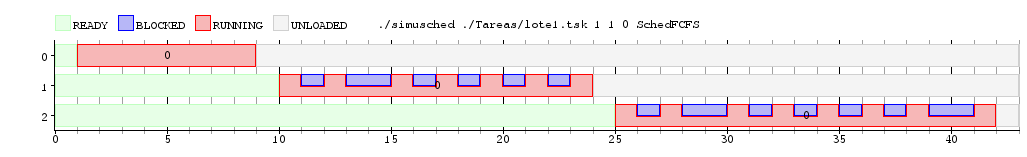
\includegraphics[width=1\textwidth]{./Graficos/ej2_1.png}
\begin{center}
 \textit{1 core}.
\end{center}

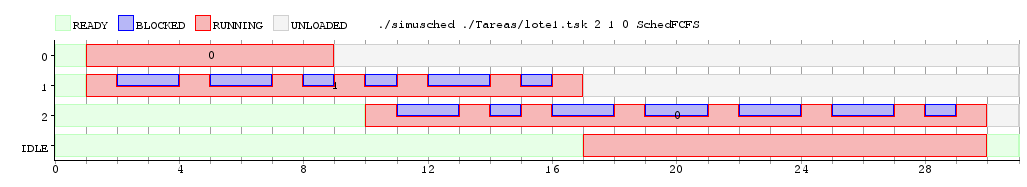
\includegraphics[width=1\textwidth]{./Graficos/ej2_2.png}
\begin{center}
 \textit{2 cores}.
\end{center}

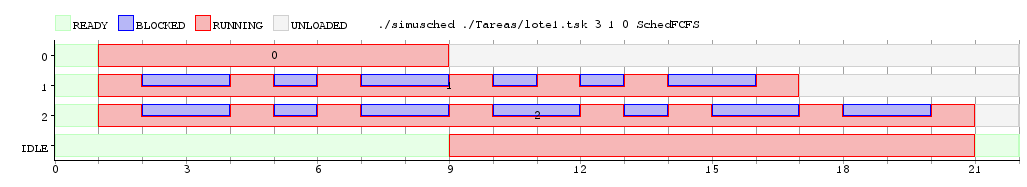
\includegraphics[width=1\textwidth]{./Graficos/ej2_3.png}
\begin{center}
 \textit{3 core}.
\end{center}

\newpage
\section{Parte II: Extendiendo el simulador con nuevos schedulers}
\subsection{Introducci�n}
En esta secci�n se extiende el simulador con un nuevo algoritmo de scheduling, \textit{Round Robin}, y se lo testea con 
diversos lotes de tareas.

\subsection{Ejercicio 3}
El objetivo de este ejercicio es implementar la pol�tica de scheduling \textit{Round Robin}. La funci�n m�s importante es \texttt{tick(cpu, motivo)}, cuya implementaci�n se 
describe a continuaci�n: si el motivo es \textbf{TICK} o \textbf{BLOCK}, se aumenta el contador de ticks del core correspondiente. Si este contador supera el quantum del core, se 
vuelve a poner el contador en $0$, se encola la tarea actual y comienza a ejecutarse la siguiente tarea en la cola; caso contrario, se sigue ejecutando la tarea actual.

Si el motivo es \textbf{EXIT}, sencillamente se devuelve la proxima tarea en la cola, sin encolar nuevamente la tarea actual. En caso de no haber m�s tareas, se ejecuta \textbf{IDLE\_TASK}.

Para m�s detalles, consultar la implementaci�n en el archivo \textit{sched\_rr.cpp}.

\subsection{Ejercicio 4}
En esta parte nos vamos a focalizar en la utilizaci�n de la pol�tica de scheduling implementada anteriormente para mostrar c�mo se comporta la misma con diversos quantums y cantidad de cores. La intenci�n es mostrar cuan eficiente o ineficiente puede ser una misma pol�tica tan solo con variar el quantum y mostrar que la elecci�n del mismo es muy importante.
Para tal motivo vamos a usar el lote \textit{lote\_ej4.tsk} que contiene 4 tareas intensas en CPU y 3 interactivas. Las de CPU llegan en el momento $0$, luego una interactiva en el momento $2$ y otras dos mas en el momento $8$.

Como primer pol�tica vamos a tomar un RR con quantum 3, y costo de cambio de contexto de 0, con s�lo un core.

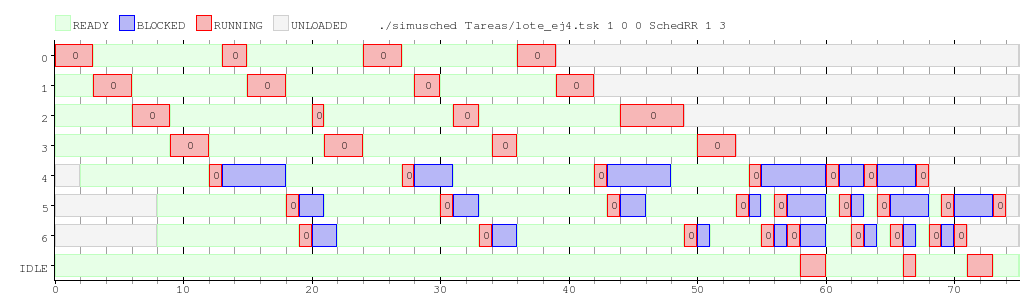
\includegraphics[width=1\textwidth]{./Graficos/ej4_1.png}
\begin{center}
 \textit{Cores = 1, Quantum = 3, CS = 0}.
\end{center}

Como podemos apreciar, se ejecutan en una primera pasada las tareas de cpu (de la 0 a la 3 inclusive) que no son interrumpidas. 

\subsection{Ejercicio 5}

Para el ejercicio 5 se nos pidi\'o dise\~nar e implementar un algoritmo de \textit{scheduling} basado en la publicaci\'on de Waldspurger, C.A. y Weihl, W.E llamada \textit{Lottery scheduling: Flexible proportional-share resource management}.

\subsubsection{Introducci\'on}

El algoritmo de \textit{Lottery scheduling} establece un sistema de prioridad para la obtenci\'on de los recursos del sistema por parte de los procesos, basado en \textit{tickets} de loter\'ia. Cada proceso es due\~no de una determinada cantidad de tickets. En cada elecci\'on de un nuevo proceso a correr por parte del scheduler, se realiza una loter\'ia entre todos los tickets del sistema, eligi\'endose uno al azar. El pr\'oximo proceso a correr es el due\~no del ticket ganador, quien se ejecutar\'a hasta la finalizaci\'on del \textit{quantum}, y el proceso se repite.

\subsubsection{Asignaci'on de recursos}

La distribuci\'ion de los tickets y posterior elecci\'on aleatoria de uno de ellos establece un sistema de prioridades probabil\'istico basado en la cantidad de tickets que posee cada proceso. Por ejemplo, sean A y B dos procesos en un sistema de 100 tickets, teniendo A 75 tickets y B 25, se esperar\'ia que el proceso A posea el 75\% de los recursos del sistema y B el 25\%. Dado el car\'acter no determin\'istico del algoritmo, no es posible confirmar que esto suceda para cualquier ejecuci\'on de las tareas. Pero la probabilidad de que esto suceda aumenta conforme a la cantidad de ejecuciones, como se mostrar\'a en la secci\'on de experimentaci\'on. Dada que la asignaci\'on de recursos esperada es proporcional a la cantidad de tickets que posee cada proceso, decimos que \textit{Lottery Scheduling} es probabil\'isticamente justo.

Los tickets \textit{encapsulan} la gesti\'on de la asignaci\'on de los recursos del sistema, ya que cuantifican la posesi\'on de \'estos por parte de los procesos independientemente de los detalles de la m\'aquina. Dado que en un determinado sistema puede haber diversos recursos heterog\'eneos, realizan una abstracci\'on uniforme de \'estos ya que la probabilidad de asignaci\'on de cualquiera de ellos a un proceso se representa homog\'eneamente a trav\'es de tickets. 

Esta representaci\'on facilita tambi\'en los cambios de prioridad entre los determinados procesos.

\textit{Nota: Dado que el \'unico recurso de sistema que se gestiona en nuestra implementaci\'on del scheduler es el tiempo de CPU, de ahora en m\'as solo nos referiremos a \'este.}

\subsubsection{Optimizaciones}

El concepto b\'asico de \textit{Lottery Scheduling} puede mejorarse considerablemente mediante la implementaci\'on de algunos mecanismos, explicados a continuaci\'on:

\begin{itemize}

\item \textit{Transferencia de tickets:} cuando un proceso est\'a bloqueado esperando la respuesta de otro proceso, puede transferir sus tickets a \'este, causando una mejora de perfomance ya que va a tener m\'as probabilidad de obtener el CPU, agilizando la respuesta. Cuando el primer proceso recibe la respuesta, le son devueltos sus tickets. De esta forma se resuelve el problema de la proridad inversa, de una manera similar a herencia de prioridades.

\item \textit{Tickets compensatorios:} los procesos que se bloquean en espera de una respuesta externa y no consumen el total de su quantum terminan obteniendo menos tiempo de CPU del que les corresponde, rompiendo el modelo de asignaci\'on en cuanto a la probabilidad. La forma de solucionar esto es la asignaci\'on de tickets compensatorios a estos procesos. De esta forma cuando un proceso utiliza una fraci\'on de su quantum, recibir\'a tickets aumentando su probabilidad de ser elegido para el pr\'oximo quantum.

\item \textit{Inflaci\'on de tickets:} cuando un proceso sabe que debe ejecutar una secci\'on cr\'itica y considera que va a necesitar m\'as tiempo de CPU, puede aumentar su n\'umero de tickets. Esta es una forma simple y eficiente de reflejar esa necesidad en el sistema, y no es necesario comunicarse con los otros procesos. Cabe aclarar que, este m\'etodo s\'olo es utilizable en un sistema donde los procesos ejecutan de forma cooperativa. 

\end{itemize}

\subsubsection{Resumen: Ventajas de Lottery Scheduling}

\begin{itemize}

\item Implementaci\'on sencilla y eficiente.

\item Provee encapsulaci\'on abstracta, relativa y uniforme de los recursos.

\item El usuario puede realizar la distribuci\'on de tickets entre sus procesos, estableciendo prioridades.

\item Realiza una distribuci\'on de los procesos probabil\'isticamente justa. 

\item La randomizaci\'on es una elecci\'on r\'apida, f\'acil de implementar, independiente de las anteriores y libre de peores casos.

\item Se puede especificar qu\'e porcentaje de procesador le corresponde a cada proceso.

\item Se resuelve el problema de la inanici\'on. Siempre y cuando un proceso tenga al menos un ticket, tiene una probabilidad no nula de ser elegido.

\item Gracias al sistema de \textit{currency}, puede implementarse un sistema modular de gesti\'on de recursos.

\item Mediante el concepto de \textit{ticket transfer}, un proceso bloqueado esperando respuesta de otro proceso puede transferir sus tickets a \'este, solucionando el problema de la prioridad inversa.


 \end{itemize}

\subsubsection{Posibles desventajas}

\begin{itemize}

\item Si bien la naturaleza aleatoria del algoritmo tiene ventajas, posee como desventaja nunca poder asegurar determin\'isticamente un resultado.

\item La asignaci\'on de los tickets a los procesos es un problema en s\'i mismo no abarcado por los autores. El comportamiento de un sistema va a depender fuertemente de la distribuci\'on de los tickets.

\end{itemize}

\subsubsection{Detalles de la implementaci\'on}

A continuaci\'on expondremos los detalles de nuestra implementaci\'on particular de \textit{Lottery Scheduling}. Dado que la probabilidad de ser asignado el CPU para cada proceso depende solamente de la cantidad de tickets que posea, y no de cu\'ales sean \'estos, no diferenciaremos entre tickets, s\'olo nos va a interesar la cantidad de tickets que posea cada proceso.


\vspace{2mm}

El sistema comienza con una cantidad de 100 tickets que son distribuidos equitativamente entre todos los procesos al comenzar, para garantizar la misma probabilidad a todos. Nuestra elecci\'on de 100 como n\'umero de tickets inicial se debe a que el c\'alculo de la probabilidad de cada proceso en base a su n\'umero de tickes es simple e inmediato, y nos provee de presici\'on suficiente. Es importante tambi\'en notar que en la experimentaci\'on, no habr\'a m\'as de 100 tareas ejecut\'andose en un mismo experimento. De todas formas la soluci\'on a esto no es m\'as que cambiar la variable por un n\'umero mayor, por ejemplo 1000.

\vspace{2mm}

La estructura de datos elegida para almacenar las tareas y su cantidad de tickets correspondiente es una lista de pares$<pid, \#tickets>$. La forma de conocer si una tarea est\'a lista para ser ejecutada es otro diccionario$<pid, bool>$, que indica, para el valor verdadero que la tarea se encuentra en estado $ready$, y para el valor falso que se encuentra en estado $block$ o $exit$.

\vspace{2mm}

\textbf{Estructuras de datos:}

\begin{itemize}

\item $int$ quantum: almacena el valor de quantum pasado por par\'ametro.

\item $int$ cantTicks: almacena la cantidad de ticks de reloj que pasaron desde el \'ultimo cambio de tarea.

\item $int$ semilla: almacena la semilla pseudoaleatoria

\item $list<pid, cantTickets>$ tareasYTickets: lista que almacena las tareas del sistema y para cada una, la cantidad de tickets que posee

\item $map<tarea, bool>$ bloqueadasTerminadas: diccionario que indica para cada tarea si se encuentra lista para ejecutar.

\end{itemize}


\vspace{2mm}

Nuestra clase scheduler recibe como par\'ametros el quantum y la semilla pseudoaleatorioa. \textit{SchedLottery} hereda de la clase \textit{SchedBase},y por lo tanto implementa las funciones \textit{load()}, \textit{unblock()} y \textit{tick()}, adem\'as cuenta con:


\vspace{2mm}

\textbf{Funciones}

\begin{itemize}

\item $load():$ carga una nueva tarea que llega al scheduler, agreg\'andola a ambos diccionarios, y repartiendo nuevamente los tickets entre todos los procesos de forma equitativa.

\item $unblock(): $ desbloquea una tarea, actualizando su valor en el diccionario bloqueadasTerminadas.

\item $tick(): $ se ejecuta en cada tick del reloj, incrementando en $1$ la cantidad de ticks de la tarea actual. En caso de que se agote el quantum de \'esta, se desaloja y se llama a loter\'ia. Si la tarea se bloque\'o se actualiza en el diccionario bloqueadasTerminadas y se llama a loter\'ia. Si la tarea En caso de que no queden m\'as tareas a ejecutar, finaliza la ejecuci\'on pasando a la tarea IDLE\_TASK.
\item $loteria(): $ se realiza la loter\'ia, eligiendo la nueva tarea a ejecutar. Se explica a continuaci\'on.

\end{itemize}

\subsubsection{Loter\'ia}

Como mencionado anteriormente, nuestra implementaci\'on no diferencia entre tickets, solamente se tiene en cuenta la cantidad de ellos que cada proceso posee. La forma de elegir al ticket ganador, es elegir un n\'umero pseudoaleatorio entre 0 y la cantidad total de tickets. Acto seguido, se recorre el la lista de tareas, y se realiza una suma parcial de la cantidad de tickets de las tareas recorridas. Se itera por las tareas, mientras la suma parcial sea menor al n\'umero ganador. La tarea ganadora va a ser aquella en la cual la iteraci\'on termine, es decir, la primera tal que la suma parcial $+$ la cantidad de tickets de la tarea ganadora supera el numero pseudoaleatorio elegido.

\begin{center}
    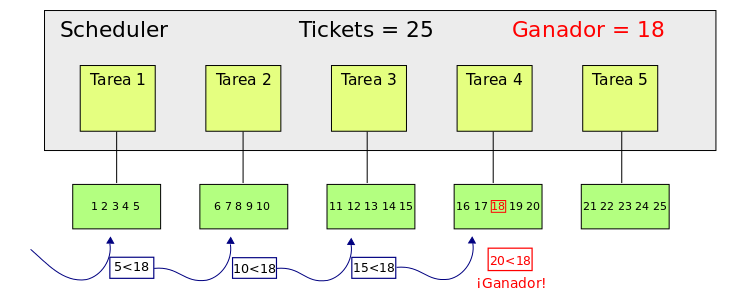
\includegraphics[scale=0.6]{./Graficos/loteria.png}
\end{center}

Dado que los tickets poseen todos el mismo valor de probabilidad, y son uniformes, de esta forma se produce una numeraci\'on autom\'atica en cada loter\'ia realizada, donde si cada tarea posee $k$ tickets, entonces sus tickets son los del intervalo de n\'umeros enteros [$sumaParcial$ .. $sumaParcial + k$].Consideramos correcta esta implementaci\'on, ya que es an\'aloga a enlistar los tickets en un vector, y en lugar de elegir el ticket de acuerdo a su n\'umero como en una loter\'ia, se eligen de acuerdo a su posici\'on en el vector (lo cual es equivalente, ya que los tickets son todos distintos y equiprobables).

\vspace{2mm}

Como por cuestiones de perfomance NO BLOQUEAMOS (NO SE)

\subsubsection{Optimizaciones}

Desde el punto de vista de performance, realizamos la optimizaci\'on sugerida por los autores para agilizar la b\'usqueda de la tarea ganadora. Esta b\'usqueda se realiza en tiempo lineal sobre la lista de tareas, buscando a la tarea due\~na del ticket ganador. Si ordenamos la lista seg\'un la cantidad de tickets de cada tarea de forma decreciente puede obtenerse una mejora de performance, ya que aquellas tareas con mayor cantidad de tickets tienen m\'as probabilidad de poseer el ticket ganador. Dado que es necesario ordenar la lista, lo realizaremos s\'olo en caso de que cambie la distribuci\'on de tickets, por ejemplo, cuando se carga una nueva tarea o cuando termina. 

\vspace{2mm}

Desde el punto de vista algor\'itmico, los autores propon\'ian diversas modificaciones que refinaban el modelo de \textit{Lottery Scheduling}. El scheduler posee la optimizaci\'on de \textbf{tickets compensatorios} previamente descripta.

\vspace{2mm}

Cuando se bloquea una tarea, nuestra implementaci\'on de los tickets compensatorios calcula la fracci\'on $f$ de quantum que \'esta utiliz\'o. Acto seguido multiplica la cantidad de tickets de la tarea por $1/f$. Como cada tarea posee la misma cantidad de tickets, ahora la tarea en cuesti\'on tiene $1/f$ m\'as probabilidad de salir que las dem\'as, siendo efectivamente compensada en la elecci\'on del siguiente quantum. HACER EXPLICACION

Las dem\'as optimizaciones no fueron consideradas por las siguientes razones:

\begin{itemize}

\item \textbf{Transferencias de tickets:} las tareas simuladas son independientes, y no se bloquean esperando una respuesta de otra tarea.

\item \textbf{Inflaci\'on de tickets:} las tareas simuladas ejecutan instrucciones fijas, en ning\'un momento ejecutan alguna secci\'on cr\'itica en la cual requieran m\'as tiempo de CPU. 

\end{itemize}



\newpage
\section{Parte III: Evaluando los algoritmos de scheduling}
\subsection{Introducci�n}
En esta secci�n se evaluan las pol��ticas de scheduling implementadas, utilizando diversas m�tricas especificadas m�s adelante.

\subsection{Ejercicio 6}
El objetivo de este ejercicio es programar un tipo de tarea \textbf{TaskBatch}, que durante \textit{total\_cpu} ciclos, realize \textit{cant\_bloqueos} llamadas bloqueantes, 
en momentos elegidos pseudoaleatoriamente. La implementaci�n consiste primero en precalcular todos los instantes en donde se van a realizar las
\textit{cant\_bloqueos} llamadas bloqueantes. Haciendo una analog�a con bolillas y urnas, si todos los posibles instantes entre el momento en que el proceso comienza a 
ejecutarse y el momento en que �ste termina de ejecutarse \textit{total\_cpu} ciclos despu�s, reprensentan las bolillas, lo que hacemos es elegir pseudoaleatoriamente
\textit{cant\_bloqueos} bolillas sin reposici�n, quedando asi determinados los momentos en los cuales se van a lanzar las llamadas bloqueantes. Luego, la tarea corre durante
\textit{total\_cpu} ciclos, utilizando la CPU o lanzando una llamada bloqueante seg�n corresponda.

Para m�s detalles, consultar la implementaci�n en \textit{tasks.cpp}.


\subsection{Ejercicio 7}

En este ejercicio debemos elegir 2 m�tricas diferentes y testear un lote de tareas \textbf{TaskBatch}, todas ellas con igual uso de CPU pero con diversas
cantidades de bloqueos. El lote de tareas utilizado es el \textit{lote3.tsk}.

Las m�tricas que elegimos fueron:
\begin{itemize}
 \item Turnaround
 \item Waiting Time 
\end{itemize}

Definidas en [Sil1] como:
\newline

\textbf{Turnaround}: Es el intervalo de tiempo entre el momento en que el proceso comienza a ejecutarse por primera vez, hasta el momento en que
el mismo termina. Es decir, es la suma de los per�odos usados en esperar datos de memoria, en estar encolado en la ``ready queue'', ejecutandose en 
la CPU, y haciendo E/S.


\textbf{Waiting Time}: Es el tiempo que un proceso se pasa encolado en la ``ready queue''.
\newline
\newline
Elegimos estas m�tricas ya que, con el Turnaround, tenemos una visi�n global de c�mo se comportan los procesos, mientras que con el Waiting Time
podemos observar c�mo un hecho m�s puntual, el tiempo que los procesos pasan encolados, impacta en el tiempo de ejecuci�n total del proceso.
\newline
\newline
Para calcular el desv�o standard utilizamos la f�rmula de [WikSD]
\newline
\newline
A continuaci�n se pueden observar los resultados de la experimentaci�n:
\newline
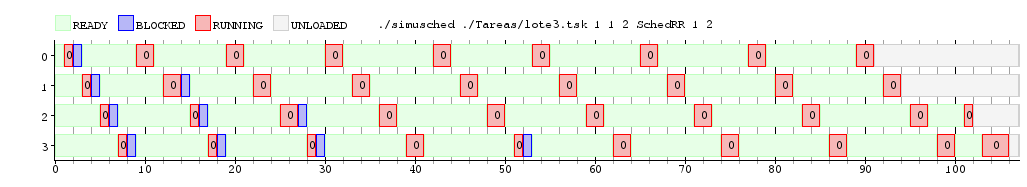
\includegraphics[width=1\textwidth]{./Graficos/ej7_1core_q2.png}
\begin{center}
 \textit{1 core, quantum = 2}.
\end{center}
~\\
\newline
Turnaround:  \hspace{7cm}  Waiting Time:

$P_{0}$: 90  \hspace{8cm}    $P_{0}$: 73

$P_{1}$: 91  \hspace{8cm}    $P_{1}$: 75

$P_{2}$: 97  \hspace{8cm}    $P_{2}$: 82

$P_{3}$: 99  \hspace{8cm}    $P_{3}$: 85


Promedio: 94,25 \hspace{6,5cm}   Promedio: 78,75


DS: 3,83         \hspace{7,7cm}    DS: 4,92
%----------------------------------------------------------------------------------------------

~\\
\newline
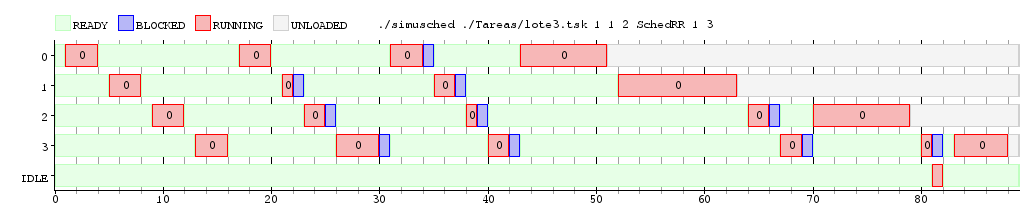
\includegraphics[width=1\textwidth]{./Graficos/ej7_1core_q3.png}
\begin{center}
 \textit{1 core, quantum = 3}.
\end{center}
~\\
\newline
Turnaround:  \hspace{7cm}  Waiting Time:

$P_{0}$: 81 \hspace{8cm}    $P_{0}$: 64

$P_{1}$: 82 \hspace{8cm}    $P_{1}$: 66

$P_{2}$: 90 \hspace{8cm}    $P_{2}$: 75

$P_{3}$: 91  \hspace{8cm}    $P_{3}$: 77


Promedio: 85,5  \hspace{6,5cm}    Promedio: 70,5


DS: 4,55        \hspace{7,6cm}    DS: 5,60
~\\
\newline


%----------------------------------------------------------------------------------------------

~\\
\newline
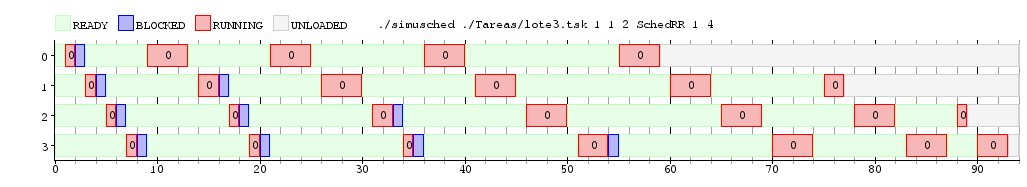
\includegraphics[width=1\textwidth]{./Graficos/ej7_1core_q4.png}
\begin{center}
 \textit{1 core, quantum = 4}.
\end{center}
~\\
\newline
Turnaround:  \hspace{7cm}  Waiting Time:

$P_{0}$: 58  \hspace{8cm}    $P_{0}$: 41

$P_{1}$: 74  \hspace{8cm}    $P_{1}$: 57

$P_{2}$: 84  \hspace{8cm}    $P_{2}$: 69

$P_{3}$: 86  \hspace{8cm}    $P_{3}$: 72


Promedio: 75,5   \hspace{6,7cm}    Promedio: 59,75


DS: 10,33         \hspace{7,5cm}    DS: 12,19
~\\
\newline




%----------------------------------------------------------------------------------------------

~\\
\newpage
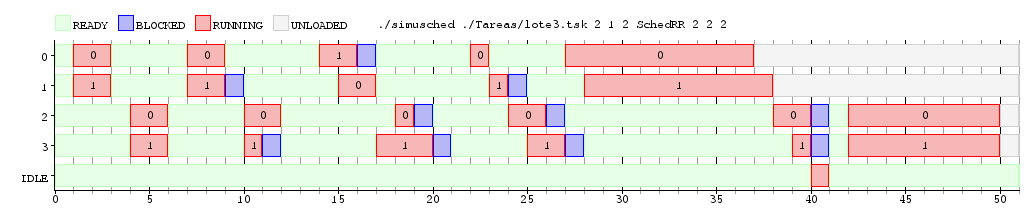
\includegraphics[width=1\textwidth]{./Graficos/ej7_2core_q2.png}
\begin{center}
 \textit{2 core, quantum = 2}.
\end{center}
~\\
\newline
Turnaround:  \hspace{7cm}  Waiting Time:

$P_{0}$: 47  \hspace{8cm}    $P_{0}$: 30

$P_{1}$: 49  \hspace{8cm}    $P_{1}$: 31

$P_{2}$: 51  \hspace{8cm}    $P_{2}$: 50

$P_{3}$: 51  \hspace{8cm}    $P_{3}$: 33


Promedio: 49,5 \hspace{6,6cm}    Promedio: 36


DS: 1,66       \hspace{7,6cm}    DS: 8,15
~\\
\newline




%----------------------------------------------------------------------------------------------

~\\
\newline
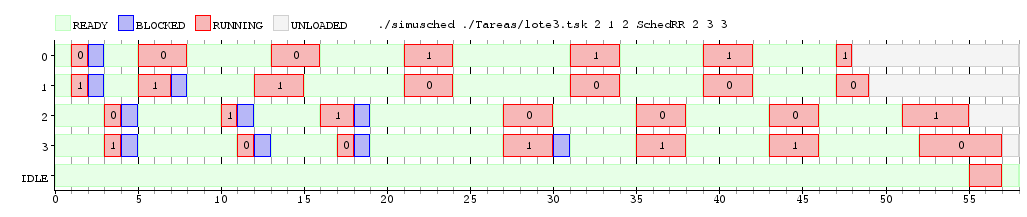
\includegraphics[width=1\textwidth]{./Graficos/ej7_2core_q3.png}
\begin{center}
 \textit{2 core, quantum = 3}.
\end{center}
~\\
\newline
Turnaround:  \hspace{7cm}  Waiting Time:

$P_{0}$: 47  \hspace{8cm}    $P_{0}$: 30

$P_{1}$: 48  \hspace{8cm}    $P_{1}$: 30

$P_{2}$: 52  \hspace{8cm}    $P_{2}$: 35

$P_{3}$: 54  \hspace{8cm}    $P_{3}$: 36


Promedio: 50,25  \hspace{6,4cm}    Promedio: 32,75


DS: 2,86         \hspace{7,6cm}    DS: 2,77
~\\
\newline




%----------------------------------------------------------------------------------------------

~\\
\newpage
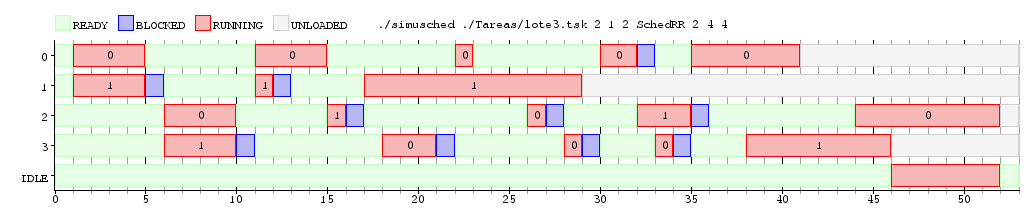
\includegraphics[width=1\textwidth]{./Graficos/ej7_2core_q4.png}
\begin{center}
 \textit{2 core, quantum = 4}.
\end{center}
~\\
\newline
Turnaround:  \hspace{7cm}  Waiting Time:

$P_{0}$: 35  \hspace{8cm}    $P_{0}$: 18

$P_{1}$: 45  \hspace{8cm}    $P_{1}$: 27

$P_{2}$: 48  \hspace{8cm}    $P_{2}$: 31

$P_{3}$: 53  \hspace{8cm}    $P_{3}$: 35


Promedio: 45,25  \hspace{6,5cm}    Promedio: 27,75


DS: 6,57        \hspace{7,6cm}    DS: 6,30
~\\
\newline


%----------------------------------------------------------------------------------------------

~\\
\newline
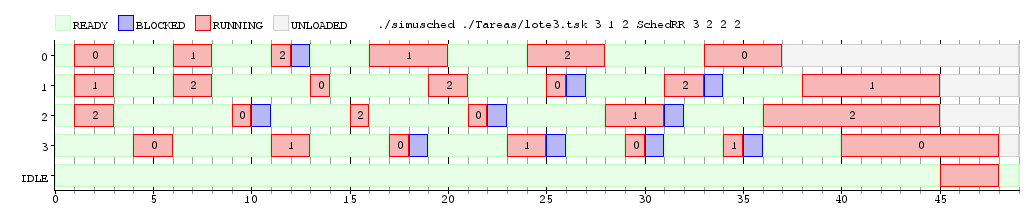
\includegraphics[width=1\textwidth]{./Graficos/ej7_3core_q2.png}
\begin{center}
 \textit{3 core, quantum = 2}.
\end{center}
~\\
\newline
Turnaround:  \hspace{7cm}  Waiting Time:

$P_{0}$: 43  \hspace{8cm}    $P_{0}$: 26

$P_{1}$: 47  \hspace{8cm}    $P_{1}$: 29

$P_{2}$: 49  \hspace{8cm}    $P_{2}$: 30

$P_{3}$: 49  \hspace{8cm}    $P_{3}$: 31


Promedio: 47  \hspace{6,9cm}    Promedio: 29


DS: 2,45          \hspace{7,6cm}    DS: 1,87
~\\
\newline



%----------------------------------------------------------------------------------------------

~\\
\newpage
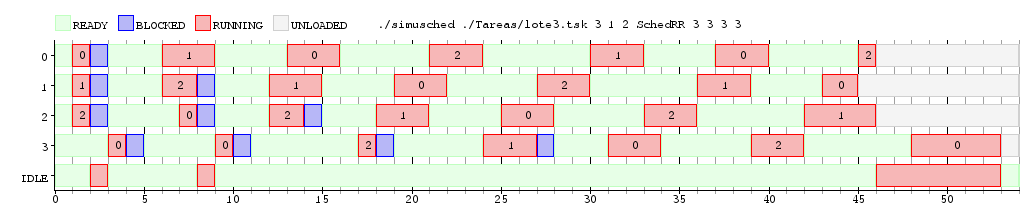
\includegraphics[width=1\textwidth]{./Graficos/ej7_3core_q3.png}
\begin{center}
 \textit{3 core, quantum = 3}.
\end{center}
~\\
\newline
Turnaround:  \hspace{7cm}  Waiting Time:

$P_{0}$: 45  \hspace{8cm}    $P_{0}$: 28

$P_{1}$: 44  \hspace{8cm}    $P_{1}$: 26

$P_{2}$: 45  \hspace{8cm}    $P_{2}$: 26

$P_{3}$: 50  \hspace{8cm}    $P_{3}$: 32


Promedio: 46   \hspace{6,9cm}    Promedio: 28


DS: 2,34        \hspace{7,6cm}    DS: 2,45
~\\
\newline



%----------------------------------------------------------------------------------------------

~\\
\newline
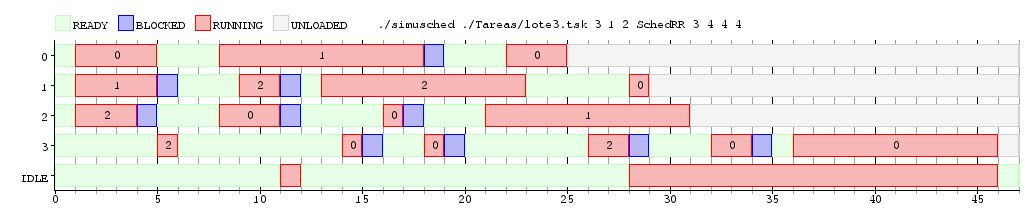
\includegraphics[width=1\textwidth]{./Graficos/ej7_3core_q4.png}
\begin{center}
 \textit{3 core, quantum = 4}.
\end{center}
~\\
\newline
Turnaround:  \hspace{7cm}  Waiting Time:

$P_{0}$: 28  \hspace{8cm}    $P_{0}$: 11

$P_{1}$: 35  \hspace{8cm}    $P_{1}$: 17

$P_{2}$: 36  \hspace{8cm}    $P_{2}$: 17

$P_{3}$: 39  \hspace{8cm}    $P_{3}$: 21


Promedio: 34,5  \hspace{6,6cm}    Promedio: 16,5


DS: 4,03          \hspace{7,6cm}    DS: 3,57 
~\\
\newline


Las conclusiones que pudimos sacar fueron las siguientes:

\begin{itemize}
 \item Dada una cantidad $i$ de cores, a medida que se aumenta el quantum, el tiempo promedio de Turnaround y Waiting Time disminuye. Esto en principio
 indicar�a que es buena idea aumentar el quantum, pero sin embargo a medida que se aumenta este, aumenta tambi�n el desv�o est�ndar, lo cual implica que los valores
 de Turnaround y Waiting Time se encuentran m�s dispersos. Esto significa que va a haber procesos que terminen relativamente r�pido mientras que otros no, lo cual disminuye
 el \textit{fairness} del sistema.
 \item Dado un mismo valor de quantum, aumentar la cantidad de cores siempre disminuye el tiempo promedio de Turnaround y Waiting Time, manteniendo o 
 reduciendo a su vez el desv�o est�ndar. Por lo tanto, obviamente, un aumento en la cantidad de cores siempre es beneficioso.
 \item El Waiting Time representa una parte muy importante del Turnaround: aproximadamente un 81\% en el caso de 1 core, 65\% con 2 cores, y 53\% con 3 cores.
 \item L�gicamente, los procesos que m�s llamadas bloqueantes realizan son los que m�s tiempo tardan en terminar. Sin embargo, en la mayor parte de los casos, 
 la diferencia en los valores de Turnaround no es demasiado significativa.
 \item El valor �ptimo del quantum para ambas m�tricas ser�a $4$, si se tolera el desv�o est�ndar asociado.
\end{itemize}


\subsection{Ejercicio 8}
En la presente secci�n vamos a trabajar sobre un algoritmo de scheduling de tipo Round Robin pero que no permite la migraci�n de procesos entre
n�cleos. Para tal motivo se utiliza una cola de \texttt{READY} para cada core, donde una vez que el proceso llega se moviliza s�lo por esa cola.

Cuando el proceso es bloqueado debemos tener una manera de saber a qu� CPU pertenec�a dicho proceso, y para tal fin cada core tambi�n tiene una
cola de \texttt{BLOQUED}. Entonces, cuando un proceso es desbloqueado simplemente se lo busca en alguna de las listas \texttt{BLOQUED} de los cores,
y una vez que se lo encuentra se lo agrega a la cola \texttt{READY} correspondiente al core que ten�a esa tarea bloqueada. Esto hace que cada CPU
tenga un esquema de Round Robin de un s�lo core independiente del resto.

A continuaci�n mostramos un gr�fico correspondiente al procesamiento del lote de tareas \textit{lote5.tsk} para este nuevo scheduler.
Las tareas se encolan acorde a su momento de llegada y a la carga de los dem�s cores. Las tres primeras se cargan una en cada core, la cuarta
se carga en el primer core ya que todos estan igualmente cargados. Luego todas siguen ejecut�ndose en sus respectivos cores sin cambios de
lugar como es esperado.


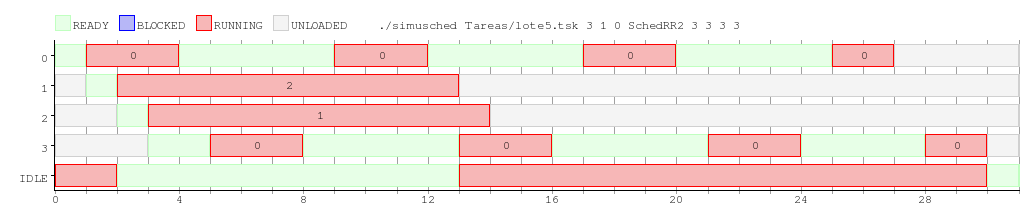
\includegraphics[width=1\textwidth]{./Graficos/ej8_1.png}
\begin{center}
 \textit{Cores = 3, Qantum = 3 cada core, CS = 1}.
\end{center}

Ahora, con el objetivo de comparar con la pol�tica de scheduling de una sola cola, vamos a correr el mismo lote para ver c�mo se comporta.
A continuaci�n se encuentra el gr�fico con la distribuci�n de las tareas.

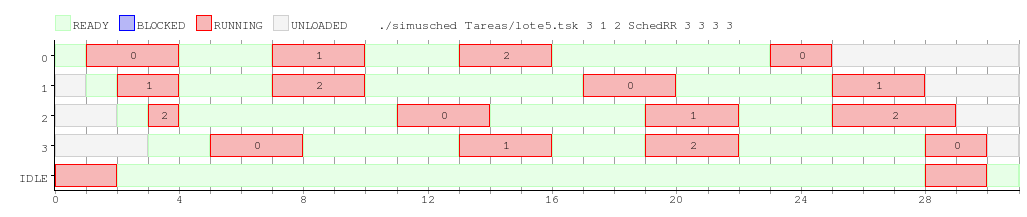
\includegraphics[width=1\textwidth]{./Graficos/ej8_2.png}
\begin{center}
 \textit{Cores = 3, Qantum = 3 cada core, CS = 1, CI = 2}.
\end{center}

Un detalle que vale la pena mencionar es que las tareas desde que iniciar hasta que finalizar estan asociadas a un solo core en el caso del
grafico uno. No ocurre asi en el gr�fico 2, en donde porciones de la tarea van cambiando de core, como se ve en el segundo gr�fico.

Para este lote de tareas en particular podemos apreciar que \texttt{SchedRR2} y \texttt{SchedRR} finalizan la ejecuci�n de todas las tareas
en un tiempo similar. Pero en el primer caso dos de las tareas finalizan r�pido, algo que no sucede en el segundo caso, sin contar que en
\texttt{SchedRR2} no hay costos por cambio de core, que s� presenta \texttt{SchedRR}.

Por otro lado, si bien es cierto que \texttt{SchedRR2} termina dos de las tres tareas m�s r�pido, tambi�n es cierto que esos cores quedan
inactivos el resto del tiempo (para este lote) algo que no es deseable. Esta comparativa nos brinda un indicio de que si bien \texttt{SchedRR2}
parece m�s eficiente, para algunos escenarios puede presentar desventajas con respecto a \texttt{SchedRR}, y dicho escenario es cuando
un core se queda con muchas tareas pendientes y los dem�s no poseen ninguna. Para estos casos se podr�a implementar alguna pol�tica de balance
de carga, es decir, si un core tiene muchas tareas y los dem�s ninguna, se podr�an mover algunas tareas del core m�s ocupado para los de menos
carga. En este caso estar�amos pagando la penalizaci�n del cambio de core (por el traslado de colas), pero es preferible eso antes que alg�n
core quede inactivo.

A continuaci�n vamos a correr nuevamente los dos schedulers con el lote de tareas \texttt{lote6.tsk} que resultar� en tareas pesadas para
el core 0, y tareas mas livianas para el resto. El primer core tendr� un quantum mas grande que los otros. La idea es mostrar un escenario
en donde puedo aprovechar cierta caracter�stica de los cores.

La idea detr�s del dise�o de este lote es construirlo para que el core 0 tome las tareas mas pesadas (en cuanto a CPU) y el resto las m�s
livianas. Adem�s se configura la corrida del scheduler con tres cores, de los cuales el primero tiene un quantum mas alto que los dem�s.
As� queda el procesamiento del \texttt{lote6.tsk} con \texttt{SchedRR2}:

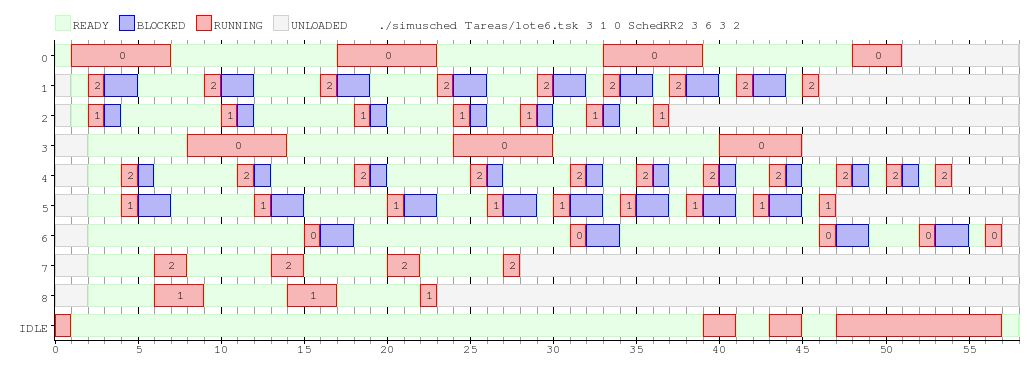
\includegraphics[width=1\textwidth]{./Graficos/ej8_3.png}
\begin{center}
 \textit{Cores = 3, Qantum = 3 cada core, CS = 1}.
\end{center}

Y con \texttt{SchedRR} el procesamiento de dicho lote queda de la siguiente forma:

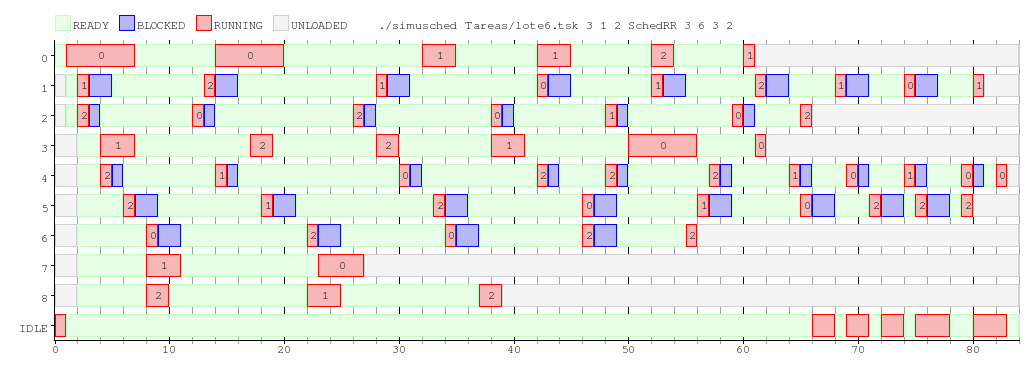
\includegraphics[width=1\textwidth]{./Graficos/ej8_4.png}
\begin{center}
 \textit{Cores = 3, Qantum = 3 cada core, CS = 1, CI = 2}.
\end{center}

Vemos que para este lote, \texttt{SchedRR2} tiene mejor performance. Las tareas son finalizadas m�s r�pido, y todo el lote es procesado
m�s r�pido que en \texttt{SchedRR}. A�n as� en \texttt{SchedRR2} tenemos bastante tiempo de procesamiento en donde un procesador u otro permanece ocioso.
Eso ocurre tambi�n en \texttt{SchedRR} pero es menor la cantidad de tiempo que los cores permanecen ociosos, aunque el desempe�o final es peor.

\section{Ejercicio 9}
En esta parte del trabajo vamos a analizar la \textit{fairness} del algoritmo de scheduling
\texttt{SchedLottery}. Tomamos como definici�n de \textit{fairness} al hecho de que cada
proceso reciba igual cantidad de tiempo de CPU, o m�s precisamente, un tiempo apropiado para
cada proceso de acuerdo a su prioridad y carga de trabajo.

A continuaci�n vamos a mostrar los experimentos realizados para poder ver que efectivamente
cuando se realizan \textit{n} experimentos, el scheduler es realmente justo cuando \textit{n} aumenta su tama�o.
Notar que es necesario hacer m�s de una corrida ya que debido al factor pseudoaleatorio del
algoritmo, realizar una o dos corridas no es suficiente para ver que efectivamente el scheduler
es justo.


\subsection{Ejercicio 10}

Dadas las implementaciones de $ShedLottery$, con o sin tickets compensatorios (respectivamente en $sched\_lottery.cpp$ y $sched\_lottery\_base.cpp$), el ejercicio nos propone ponerlas a prueba y compararlas, relacion\'andolas con la problem\'atica que presentaban los autores y verificar si los tickets compensatorios son una soluci\'on viable. 

\vspace{2mm}

Para esto generamos dos lotes distintos: \textbf{Lote7}, que consta de 3 tareas intensivas de CPU y una tarea de I/O bloqueante, y para comprobar que el mecanismo funciona con varias tareas bloqueadas al mismo tiempo, el lote \textbf{Lote8} con 2 tareas intenstivas de CPU y 2 bloqueantes.

\vspace{2mm}
\textbf{Lote7:}

\begin{lstlisting}[numbers=none]
@0:
*3 TaskCPU 50
*1 TaskConsola 50 1 2
\end{lstlisting}

\vspace{2mm}
\textbf{Lote8:}

\begin{lstlisting}[numbers=none]
@0:
*2 TaskCPU 50
*2 TaskConsola 25 1 2
\end{lstlisting}

\subsubsection{Experimentos: Lote 7}

\vspace{2mm}

Los experimentos fueron realizados con los par\'ametros: \textbf{semilla} aleatoria(pero la misma para cada comparaci\'on entre schedulers), \textbf{quantum} de tres ticks, \textbf{bloqueos} de un tick (con el objetivo de generar muchos cambios de contexto y tener m\'as casos de an\'alisis), \textbf{cantidad de procesadores} de uno y costo de \textbf{cambio de contexto} de cero, para hacer m\'as sencillo el an\'alisis y no agregar variables que no aportan al experimento.

\vspace{2mm}

\textbf{Caso1:}

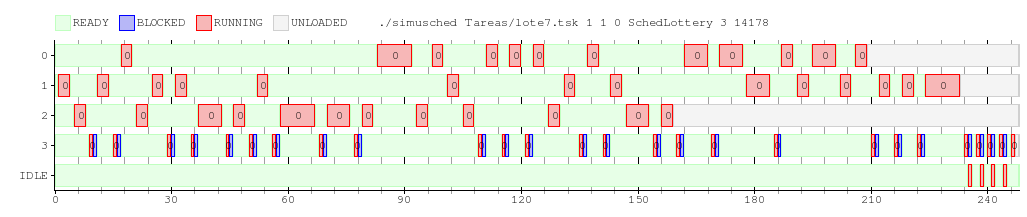
\includegraphics[width=1\textwidth]{./Graficos/Ej10v2/Task7/ej9_1.png}
\begin{center}
 \textit{Scheduler = Compensatorio, Semilla = 14178}.
\end{center}


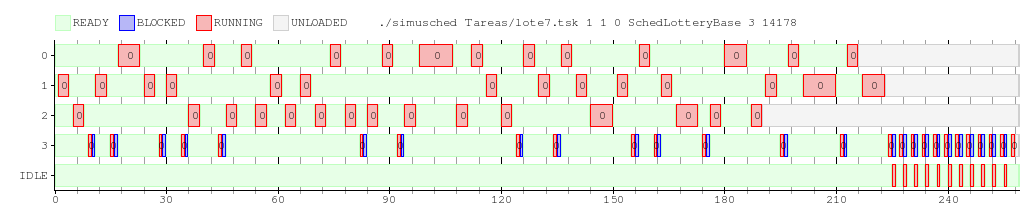
\includegraphics[width=1\textwidth]{./Graficos/Ej10v2/Task7/ej9_1_base.png}
\begin{center}
 \textit{Scheduler = No Compensatorio, Semilla = 14178}.
\end{center}

\vspace{2mm}


Pueden notarse las 3 tareas intensivas de CPU y la tarea I/O, que procesa 1 tick y se bloquea. Aqui vemos como, en el caso sin compensation tickets, la tarea se bloquea, perdiendo $2/3$ de su quantum y luego vuelve a obtener el cpu muchos ticks despues, perdiendo tiempo de procesamiento. Esto se nota claramente al ver que m\'as de la mitad de su tiempo de procesamiento se produce al final de la simulaci\'on.

\vspace{2mm}

En el caso con compensation tickets, puede notarse como luego de bloquearse, en el siguiente cambio de contexto a su desbloqueo vuelve a obtener la cpu en varios casos, producto de su aumento de probabilidad gracias a los compensation tickets. Pueden compararse adem\'as ambos finales de las simulaciones y notar que, en la simulaci\'on con tickets compensatorios, restan muchos menos ticks de la tarea I/O por procesar.

\vspace{2mm}
\textbf{Caso2:}

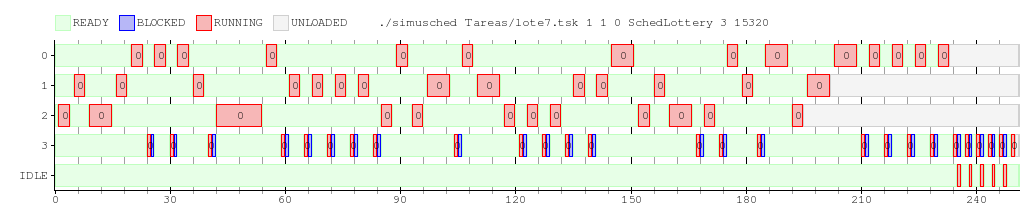
\includegraphics[width=1\textwidth]{./Graficos/Ej10v2/Task7/ej9_2.png}
\begin{center}
 \textit{Scheduler = Compensatorio, Semilla = 15320}.
\end{center}


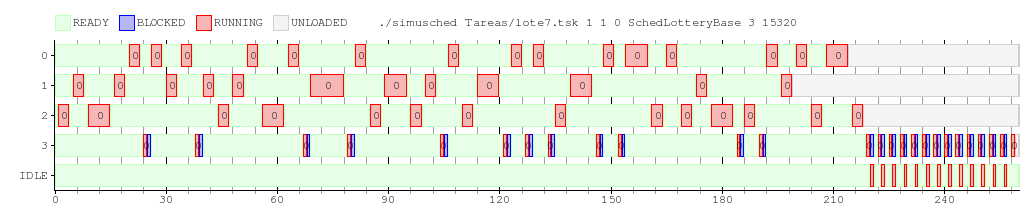
\includegraphics[width=1\textwidth]{./Graficos/Ej10v2/Task7/ej9_2_base.png}
\begin{center}
 \textit{Scheduler = No Compensatorio, Semilla = 15320}.
\end{center}

En este caso pueden observarse tambi\'en bursts de la tarea I/O, y puede notarse adem\'as que una vez que la tarea pierde la asignaci\'on de la CPU en su tick compensado, es poco probable que la vuelva a obtener por un per\'iodo, ya que debido a la implementaci\'on de tickets compensatorios, si una tarea compensada pierde la asignac\'on, sus tickets compensatorios son retirados de todas formas.

\vspace{2mm}
\textbf{Caso3:}


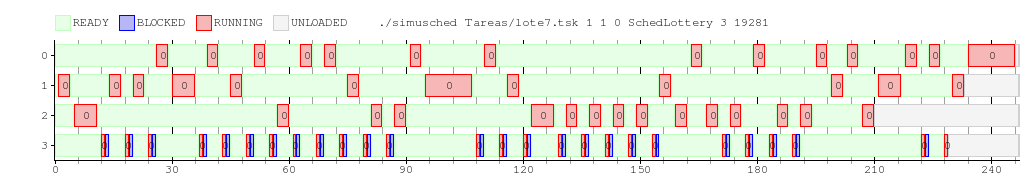
\includegraphics[width=1\textwidth]{./Graficos/Ej10v2/Task7/ej9_3.png}
\begin{center}
 \textit{Scheduler = Compensatorio, Semilla = 19281}.
\end{center}


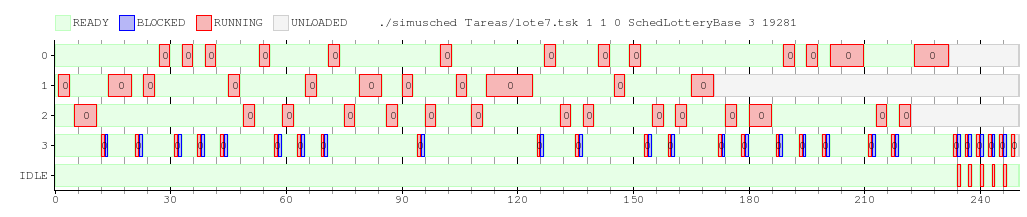
\includegraphics[width=1\textwidth]{./Graficos/Ej10v2/Task7/ej9_3_base.png}
\begin{center}
 \textit{Scheduler = No Compensatorio, Semilla = 19281}.
\end{center}

En este caso se aprecia claramente que la implementaci\'on de tickets compensatorios equilibra efectivamente la asignaci\'on de CPU, ya que comparado con la simulaci\'on no compensada, donde la tarea I/O debe terminar su ejecuci\'on al \'ultimo, en el caso compensado esta tarea recibe la asignaci\'on del CPU mucho m\'as frecuentemente, e incluso finaliza su ejecuci\'on \textbf{antes} que dos de las dem\'as.

\vspace{2mm}
\textbf{Caso4:}


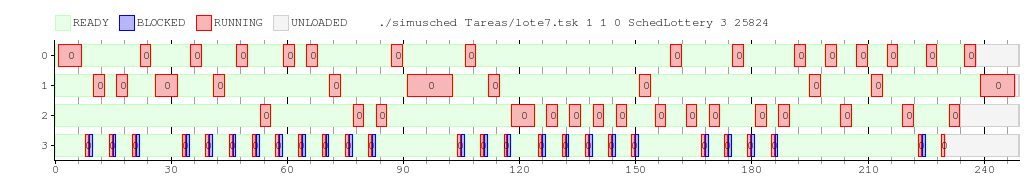
\includegraphics[width=1\textwidth]{./Graficos/Ej10v2/Task7/ej9_4.png}
\begin{center}
 \textit{Scheduler = Compensatorio, Semilla = 25824}.
\end{center}


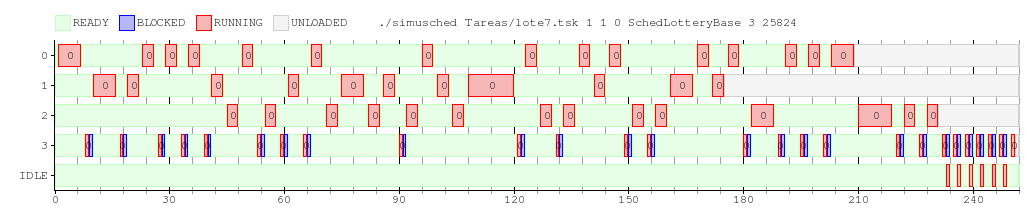
\includegraphics[width=1\textwidth]{./Graficos/Ej10v2/Task7/ej9_4_base.png}
\begin{center}
 \textit{Scheduler = No Compensatorio, Semilla = 25824}.
\end{center}

El \'ultimo caso analizado refleja correctamente todo lo anteriormente planteado. De esta forma concluimos en que en el caso de una tarea que se bloquea frecuentemente y compite por el CPU contra varias otras de uso intensivo de \'este, la implementaci\'on de tickets compensatorios logra homogeneizar la asignaci\'on y aprovechar ciclos de procesamiento.

\subsubsection{Experimentos: Lote 8}

\vspace{2mm}

Con el lote 8 analizamos si el mecanismo se mantiene eficiente cuando hay m\'as de una tarea I/O en ejecuci\'on.

\vspace{2mm}


\textbf{Caso1:}

\vspace{2mm}

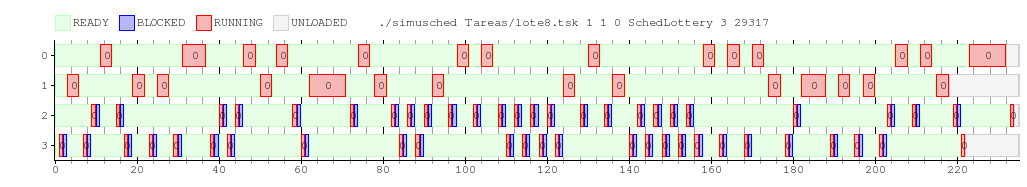
\includegraphics[width=1\textwidth]{./Graficos/Ej10v2/Task8/ej9_3.png}
\begin{center}
 \textit{Scheduler = Compensatorio, Semilla = 29317}.
\end{center}


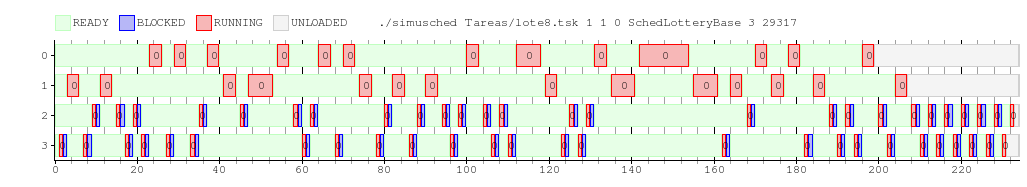
\includegraphics[width=1\textwidth]{./Graficos/Ej10v2/Task8/ej9_3_base.png}
\begin{center}
 \textit{Scheduler = No Compensatorio, Semilla = 29317}.
\end{center}

\vspace{2mm}

A primera vista puede notarse que el mecanismo contin\'ua siendo eficiente, ya que en el modo compensado las tareas I/O terminan junto con las dem\'as, en cambio en el modo no compensado finalizan \'ultimas.
\vspace{2mm}

\textbf{Caso2:}

\vspace{2mm}

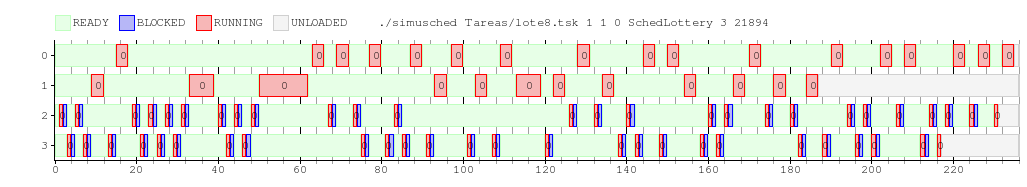
\includegraphics[width=1\textwidth]{./Graficos/Ej10v2/Task8/ej9_4.png}
\begin{center}
 \textit{Scheduler = Compensatorio, Semilla = 21894}.
\end{center}


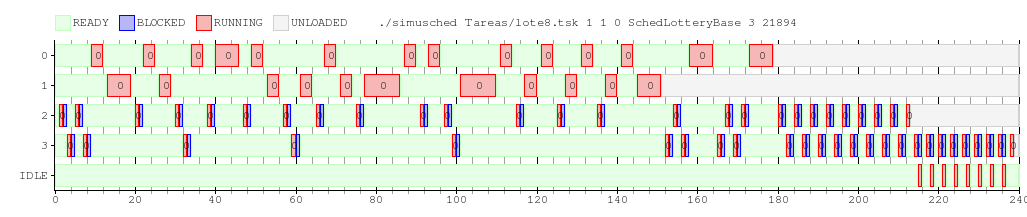
\includegraphics[width=1\textwidth]{./Graficos/Ej10v2/Task8/ej9_4_base.png}
\begin{center}
 \textit{Scheduler = No Compensatorio, Semilla = 21894}.
\end{center}

\vspace{2mm}


En este caso es a\'un m\'as notoria la tendencia, ya que en el modo no compensado las tareas I/O poseen casi todo su tiempo de procesamiento al final, en cambio en el modo compensado todas las tareas finalizan aproximadamente al mismo momento. Puede apreciarse como se aprovechan ticks de CPU, simplemente con ver la escala de ticks. Esto muestra que es eficiente priorizar la asignaci\'on de CPU a las tareas que se bloquean constantemente, ya que consumen poco tiempo de CPU y vuelven a bloquearse, trasfiriendo la CPU a otras tareas. De otra forma son relegadas hasta el final de la ejecuci\'on, y en sus bloqueos ya no quedan tareas y se debe switchear a la tarea IDLE.

\vspace{2mm}

\textbf{Caso3:}

\vspace{2mm}

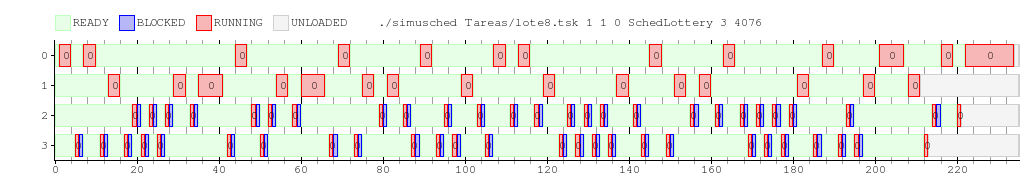
\includegraphics[width=1\textwidth]{./Graficos/Ej10v2/Task8/ej9_5.png}
\begin{center}
 \textit{Scheduler = Compensatorio, Semilla = 4076}.
\end{center}


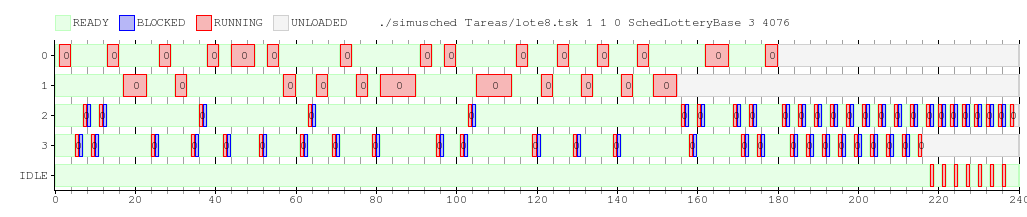
\includegraphics[width=1\textwidth]{./Graficos/Ej10v2/Task8/ej9_5_base.png}
\begin{center}
 \textit{Scheduler = No Compensatorio, Semilla = 4076}.
\end{center}

\vspace{2mm}

Con este caso finalizamos el an\'alisis. ya que consideramos que los resultados son claros y que el mecanismo de compensation tickets, tal como lo describen los autores es muy efectivo en solucionar la problem\'atica de la asignaci\'on justa del CPU para aquellas tareas que se bloquean y no consumen su quantum entero. Mediante los compensation tickets, no s\'olo se vuelve m\'as justa la asignaci\'on, sino que tambi\'en se aprovechan ticks de procesamiento.


\newpage
\section{Referencias}
[Sil1] A. Silberschatz, \textit{Operating System Concepts, 4� Ed., 1994}
\end{document}
